\documentclass[11pt]{article}

\usepackage{titlesec}
\usepackage[hidelinks]{hyperref}
\usepackage{titling}
\usepackage[margin=1in,headheight=0pt,headsep=0pt]{geometry}
\usepackage{multicol}
\usepackage{graphicx}
\usepackage{tcolorbox}
\usepackage{multirow}
\usepackage{makecell}
\usepackage{xcolor}
\usepackage{titlesec}
\usepackage{pifont} % bullet points for itemize
\usepackage{enumitem} % packed itemize


\definecolor{mycolor}{rgb}{0.122, 0.435, 0.698}% Rule colour

% Reduce the margin from the top of the page
\setlength{\voffset}{-0.5in}
\setlength{\headsep}{5pt}


% Format some parts
\titleformat{\section}
{\Large\bfseries\uppercase}
{}
{0em}
{}[\titlerule]

\titleformat{\subsection}
{\bfseries\Large}
{$\bullet$}
{0em}
{}

\titleformat{\subsubsection}
{\bfseries}
{}
{0em}
{}

\newtcbox{\topic}{on line,
colframe=mycolor,
colback=mycolor!10!white,
boxrule=0.5pt,
arc=4pt,
boxsep=0pt,
left=6pt,
right=6pt,
top=6pt,
bottom=6pt}

\newtcbox{\nameTitleBox}{on line,
colframe=gray,
colback=white,
boxrule=1pt,
arc=2pt,
boxsep=0pt,
left=6pt,
right=6pt,
top=6pt,
bottom=6pt}

% define function
% arguments: level, place, graduation, image
\newcommand*{\eduWithDetail}[5]
{\begin{table}[h!]
	\begin{tabular*}{\textwidth}{ll@{\extracolsep{\fill}}r}
		\textbf{#1} &  #2 & \\ % \multirow{2}{*}{\includegraphics[width=40px]{#4}} \\
		#3 &  & \\
		\multicolumn{3}{l}{#5}
	\end{tabular*}
\end{table}}

\newcommand*{\eduSmall}[5]
{\begin{table}[h!]
	\begin{tabular*}{\textwidth}{ll@{\extracolsep{\fill}}r}
		\textbf{#1} &  #2 & \\ % \multirow{2}{*}{\includegraphics[width=40px]{#4}} \\
		#3 &  & \\
		\multicolumn{3}{l}{#5}
	\end{tabular*}
\end{table}}

\newcommand*{\multilineCell}[1]
{\begin{tabular}[c]{@{}l@{}} #1
\end{tabular}}

% 1: Name 2: Date 3: Lecturer 4: Level
\newcommand*{\taRecord}[4]{\textbf{#1}\quad (#3) \\ #2 \quad  #4}

\def\today{\number\day \space \ifcase\month\or
	Jan\or Feb\or Mar\or Apr\or May\or Jun\or
	Jul\or Aug\or Sep\or Oct\or Nov\or Dec\fi
	\space \number\year}

\begin{document}
% Title and Header section
% {% Image
%     \begin{minipage}[t]{100px}
%         % add a row so that contacts minipage is alligned with
%         % this line, but remove the space added for the line
%         \strut\vspace*{-\baselineskip}\newline
%         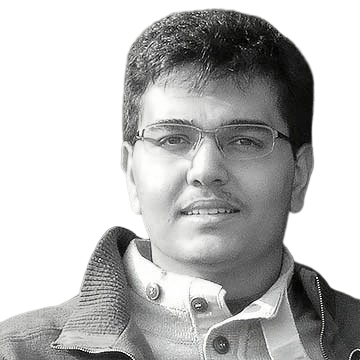
\includegraphics[width=80px]{images/farbod.png} \\
%     \end{minipage}
%     Name
%     \nameTitleBox{
%     \begin{minipage}[t]{3.5cm}
%         \vspace{8mm}
%         \noindent
%         \huge\bfseries
%         Farbod\\
%         Shahinfar
%         % \vspace{0.0cm}
%     \end{minipage}
%     }
%     \hfill\null
%     \begin{minipage}[t]{6cm}
%         \vspace{6mm}
%         % Contact Information
{ % \small
% \noindent
% \flushright
\noindent
% Phone: +989128077968 \\
\small \faEnvelope  \hspace{0.05cm}   Email: \href{mailto:iman.rahmati@sharif.edu}{iman.rahmati@sharif.edu} \space \href{mailto:imanrht@gmail.com}{imanrht@gmail.com} \\
%\faLink \hspace{0.05cm} Web page: \href{https://imanrht.github.io}{imanrht.github.io} \\
\faGithub \hspace{0.1cm} Github: \href{https://github.com/ImanRHT}{https://github.com/ImanRHT}  \\
\faLinkedin \hspace{0.1cm} Linkedin: \href{https://linkedin.com/in/iman-rahmati}{linkedin.com/in/iman-rahmati}\\
% Birthday: 25/Feb/1998 \\
}
% ===================================================================

%     \end{minipage}
% }
{\noindent \huge\bfseries Iman Rahmati}\hfill{\footnotesize updated: \today}
\vspace{-1cm}
\section{}
% Contact Information
{ % \small
% \noindent
% \flushright
\noindent
% Phone: +989128077968 \\
\small \faEnvelope  \hspace{0.05cm}   Email: \href{mailto:iman.rahmati@sharif.edu}{iman.rahmati@sharif.edu} \space \href{mailto:imanrht@gmail.com}{imanrht@gmail.com} \\
%\faLink \hspace{0.05cm} Web page: \href{https://imanrht.github.io}{imanrht.github.io} \\
\faGithub \hspace{0.1cm} Github: \href{https://github.com/ImanRHT}{https://github.com/ImanRHT}  \\
\faLinkedin \hspace{0.1cm} Linkedin: \href{https://linkedin.com/in/iman-rahmati}{linkedin.com/in/iman-rahmati}\\
% Birthday: 25/Feb/1998 \\
}
% ===================================================================
 \vspace{-2mm}

\noindent{\textbf{Research Interests:}} Distributed Systems, Mobile Edge Computing, Deep Reinforcement Learning, Federated Learning, Software Defined Networking, Performance Evaluation
\vspace{-2mm}
\section{Education}



%\vspace{-0.5cm}
%\eduWithDetail{Ph.D. Information Technology}
%{Politecnico di Milano}
%{Expected Graduation date 2026}
%{}
%{\multilineCell
%	{\hspace{5mm} \textbf{Advisor}: Prof. Gianni Antichi}
%}
\vspace{-5mm}

\eduWithDetail{MSc. Computer Software Engineering}
{Sharif University of Technology (SUT)}
{Graduated Sep 2022}
{images/sharif.png}
{\multilineCell
	{\hspace{5mm} 17.36/20 GPA (23 units) \\
        \hspace{5mm} \textbf{Thesis}:
        Optimizing Computational Task Offloading Problem in Energy-Constrained Mobile \\ 
        \hspace{21.5mm}Edge Computing Systems with Deep Reinforcement Learning\\
        \hspace{5mm} \textbf{Supervisor}: Prof. \href{https://scholar.google.com/citations?user=BXNelwwAAAAJ\&hl=en}{\textbf{Ali Movaghar}}}
}
\vspace{-5mm}

\eduWithDetail{BSc. Industrial Engineering}
{Khajeh Nasir Toosi University of Technology (KNTU)}
{Graduated Sep 2019}
{images/iust.png}
{%\multilineCell{\hspace{5mm}\vspace{-3mm} \\ %\textbf{Frist Rank}, 18.62/20 GPA \\
	%\hspace{5mm} \textbf{Project}:
	%Study of MMU Cache Partitioning Efficacy for Hierarchical Page Tables \\
	%\hspace{10mm} in OS Memory Management \\
	%\hspace{5mm} \textbf{Supervisor}: Dr. Mohsen Sharifi}
}
\vspace{-10mm}

% \eduSmall{High School Diploma}
% {Salam 3}
% {Graduated May 2015}
% {images/salam.png}
% {\hspace{5mm} \textbf{GPA:} 19.84/20}

\section{Honors}
\begin{itemize}
	\renewcommand\labelitemi{\ding{118}}
	\item{Ranked Top 25\% in the Department of Computer Engineering among M.Sc. Students, SUT, Class 2019 \hfill Jul 2022}\vspace{-2mm}
	\item {Ranked 55$^{th}$ among 30,000 Participants in the Nationwide University Entrance Exam of Computer Engineering for M.Sc. in the Field of Software Engineering \hfill Aug 2019}\vspace{-2mm}
	\item{Ranked Top 1\% among 180,000 Participants in the Nationwide University Entrance Exam for B.Sc. in the Field of Mathematics and Physics  \hfill Jul 2014}
\end{itemize}

\section{Academic Experience}

\large\large\textbf{Teaching Assistant}

\begin{itemize}

	\item \textbf{Performance Evaluation of Computer Systems (Head TA)} \hfill SUT, 2020-present
		\\ Prof. Ali Movaghar and Dr. Mahdi Dolati
	\item \textbf{Software Defined Networking (Head TA)} \hfill SUT, 2022
		\\ Prof. Ali Movaghar and Dr. Mohammad Hosseini
	\item \textbf{Verification of Reactive Systems} \hfill SUT, 2021
		\\ Prof. Ali Movaghar 
	\item \textbf{Theory of Machines and Languages} \hfill SUT, 2021
		\\ Prof. Ali Movaghar 

		
\end{itemize}
\large\large\textbf{Research Assistant}
\begin{itemize}
	\item \textbf{Research Assistant at Performance and Dependability Laboratory (PDL)}
	\\ Under the supervision of Prof. Ali Movaghar \hfill SUT, 2020-present\\
	\textbf{Research Theme:}
	\item 
	
\end{itemize}



\section {Academic Projects}

\section {Publication}
%\begin{itemize}
    %\item A. Sanaee, F. Shahinfar, B. E. Stephens, G. Antichi, ``Backdraft: a Lossless Virtual Switch that
       % Prevents the Slow Receiver Problem'', in NSDI 2022.

    %\item F. Shahinfar, S. Miano, A. Sanaee, G. Siracusano, R. Bifulco, G. Antichi,
        %``The case for network functions decomposition'', in CoNext 2021. \textbf{[BEST POSTER]}
%\end{itemize}

\section{Skills}
%\begin{itemize}[noitemsep,topsep=0pt,parsep=0pt,partopsep=0pt]
%	\item {Programming Languages: C, Python, Bash, \LaTeX}
%	\item {Frameworks \& Tools: DPDK, eBPF/XDP, AF\_XDP, Linux}
%	\item {Languages: Farsi (Native), English (Working proficiency)}
%	% \item BESS: Berkeley Extensible Software Switch
%	% \item TAS: TCP Accelartion Service
%\end{itemize}

% \subsection{Linux Programming:}
% \begin{itemize}
%     \item Linux Kernel Memory Subsystem
%     \item Developing Kernel Modules
% \end{itemize}

% \noindent \textbf{Programming Languages:}
% \begin{itemize}
%     \setlength\itemsep{0em}
%     \begin{multicols}{2}
%         \item {Python}
%         \item {C/C++}
%         \item {Javascript}
%         \item {Bash Script}
%         % \item {C\#}
%         % \item {Java}
%         % \item {SQL}
%     \end{multicols}
% \end{itemize}

% \subsection{Frameworks:}
%     \emph{React Native},
%     \emph{Flask},
%     \emph{Numpy and Matplotlib}

% \subsection{Softwares:}
% \begin{itemize}
%     \setlength\itemsep{0em}
%     \begin{multicols}{2}
%     \item{Docker}
%     \item{Git}
%     \item{PostgreSQL}
%     \item{MongoDB}
%     \item{Redis \& Memcached}
%     \item{Unity3d}
%     \item{Vim}
%     \item \LaTeX
%     \end{multicols}
% \end{itemize}

% \section {Work Experience}
% \noindent \textbf{Smart Online Monitoring Co} \par
% Mobile Application Developer \par
% January 2020 – April 2021 \par
% \begin{itemize}
%     \item Develop android application with React Native framework
%     \item Use BLE (bluetooth low energy) communication protocl
% \end{itemize}
% \topic{React Native}
% \topic{Javascript}
% \topic{BLE}
% \vspace{15pt}

% \noindent \textbf{Cognia} (DigikalaNEXT Summer Camp) \par
% Backend Developer \par
% July 2019 – March 2020 \par
% \begin{itemize}
%     \item Develop data gathering and data processing service
%     \item Deploy service with containerization
% \end{itemize}
% \topic{Python}
% \topic{Flask}
% \topic{PostgreSQL}
% \topic{Docker \& Docker Compose}
% \topic{Locust}
% \vspace{15pt}

% \noindent \textbf{Loop Game Studio} \par
% Backend Developer (A project contract) \par
% June 2019 – August 2019 \par
% \begin{itemize}
%     \item Develop a REST API server for the game.
%     \item Design a relational database for cutsomizable items in sale.
% \end{itemize}
% \topic{Python - Flask}
% \topic{PostgreSQL}
% \topic{Docker \& Docker Compose}
% \vspace{15pt}

% \noindent \textbf{ElmoGame} \par
% Game developer \par
% July 2017 – January 2019 \par
% \begin{itemize}
%     \item Work with Unity3d engine
%     \item Apply software design patterns in the project
%     \item Communicate with game server using REST APIs
% \end{itemize}
% \topic{Unity3D}
% \topic{C\#}
% \vspace{15pt}

% \section{Projects}
% \begin{multicols}{2}
% \begin{itemize}
%         \item { \emph{Footyard:} An online multi-player game developed for
%                 android devices.}
% \end{itemize}
% \end{multicols}

% \section{Languages:}
%     \emph{Persian}: Native \\
%     \emph{English}: Working Profeciency

\end{document}
